\chapter{Material und Methode}
In diesem Kapitel werden die benötigten Hilfsmittel und Techniken beschrieben, welche für die Realisierung der Applikation benötigt werden.
\section{Material}
Dieser Abschnitt beschreibt die verwendeten Software-Applikationen und deren Möglichkeiten, sowie verwendete Geräte für die Durchführung von Messungen. Weiterhin werden Evalkits beschrieben, welche für die Beschleunigung des Entwicklungsprozesses genutzt werden.
\subsection{Verwendete Programme}
%\subsubsection*{Eagle}
%\href{http://www.cadsoft.de/?language=de}{Cadsoft Eagle} ist eine \ac{pcb} Design Software, welche für Microsoft\SymbC Windows\SymbReg, Linux Distributionen sowie für Apple OS X verfügbar ist und aktuell die Versionsnummer 6.5.0 trägt. Diese Software wurde für die Erstellung eines Schaltplans, sowie für das Erstellen eines Leiterplattenlayout genutzt, was sich durch die Ableitung des zuvor erstellten Schaltplans schnell realisieren lies. Dazu stehen der Schaltplan-Editor und der Layout-Editor zur Verfügung, welche sich gegenseitig synchronisieren und Änderungen in dem jeweils anderen Editor sichtbar machen. Die Überprüfung des Leiterplattenlayout durch "Design Rules", welche man bei den gewünschten Hersteller der Platinen beziehen kann, wird bereitgestellt, wodurch die Entwicklungszeit und Fehler reduziert werden. \cite{eagle}
\subsubsection*{Altium\SymbReg Designer\SymbReg}\label{sw:altium}
\href{http://www.altium.com/de/altium-designer/overview}{Altium\SymbReg Designer\SymbReg} ist eine \ac{pcb} Design Software, welche für Microsoft\SymbC Windows\SymbReg verfügbar ist und aktuell die Versionsnummer 15.1.12 trägt. Diese Software wurde für die Erstellung eines Schaltplans, sowie für das Erstellen eines Leiterplattenlayouts genutzt, was sich durch die Ableitung des zuvor erstellten Schaltplans schnell realisieren lies. Dazu stehen der Schaltplan-Editor und der Layout-Editor zur Verfügung, welche sich gegenseitig synchronisieren und Änderungen in dem jeweils anderen Editor sichtbar machen. Die Überprüfung des Leiterplattenlayout durch \glqq Design Rules\grqq{} wird bereitgestellt, wodurch die Entwicklungszeit und Fehler reduziert werden. Dabei können diese Regeln bei den gewünschten Hersteller der Platinen bezogen werden.\cite{altium}

\subsubsection*{LTspice IV\SymbReg}\label{sw:ltspice}
\href{LTspice IV}{LTspice IV\SymbReg} ist ein hochperformanter SPICE Simulator, welcher für Microsoft\SymbC Windows\SymbReg und Mac OS X 10.7+ verfügbar ist und aktuell die Versionsnummer 4.23e trägt. Diese Software wurde von Linear Technology Corporation für die analoge Schaltungssimulation entwickelt, wodurch Sie für die Validierung des Bandpassfilters sowie der Transmitteransteuerung genutzt werden konnte. \cite{ltspice}

\subsubsection*{Lattice\SymbC Diamond\SymbReg}\label{subsub:diamond}
Diamond\SymbReg  ist eine Design Software der Firma Lattice\SymbC, welche für Microsoft\SymbC Windows\SymbReg und Linux Distributionen verfügbar ist. Diese wurde für die Erstellung von Logikmodulen (in der Programmiersprache Verilog 2.0) und die Verknüpfung der erstellten Module in einem System Design verwendet. Dieses Design konnte durch den integrierten Compiler für die Programmierung des Lattice MachXO2\SymbTM bereitgestellt, sowie übertragen werden. Dabei wurde die Version 3.4.080 verwendet.
\subsubsection*{ALDEC Active-HDL\SymbTM}\label{subsub:aldec}
Active-HDL\SymbTM ist eine Design Erstellungs- und Simulations-\ac{ide} für \acl{fpga}s (\acs{fpga}s) der Firma Aldec, welche für Microsoft\SymbC Windows\SymbReg verfügbar ist. Diese Software ist in Lattice Diamond\SymbReg integriert und wurde für die Simulation \ac{bzw} Synthese der Logikmodule und des System Designs des MachXO2\SymbTM genutzt. Die verwendete Version trägt die Nummer 9.3 und die Buildkennung 2744.sp1.09.4995.01.
%\subsubsection*{Visual Studio Ultimate}
%Visual Studio\SymbReg ist eine Software Entwicklungs \ac{ide} der Firma Microsoft\SymbC, welche unter Microsoft\SymbC Windows\SymbReg verfügbar ist. Diese \ac{ide} wird für die Code Dokumentation verwendet und bietet zusätzlich sehr gute Code Analyse Tools für die Programmiersprachen C, C++ und alle .NET Sprachen.
\subsubsection*{NXP Semiconductors LPCXpresso}\label{sec:xpresso}
\href{http://www.lpcware.com/lpcxpresso/home}{LPCXpresso} ist eine Software Entwicklungs \ac{ide} auf der Basis von Eclipse. Mit dieser Software wurde die Firmware des ARM-Cortex erstellt und gedebuggt. \cite{lpcxpresso}
\subsubsection*{Texmaker}
Bei \href{http://http://www.xm1math.net/texmaker/}{Texmaker} handelt es sich um ein Textsatzprogramm, welches von Pascal Brachet\SymbC unter Verwendung von Qt 5.2.1 sowie Poppler 0.26.5 compiliert wurde und für Microsoft\SymbC Windows\SymbReg, Linux Distributionen sowie für Apple OS X verfügbar ist. Die aktuelle Version, welche verwendet wurde trägt die Versionsnummer 4.4.1.
%\subsubsection*{Inventor}
%Als CAD-Programm wird Inventor\SymbReg Professional 2014 verwendet. Dieses, von Autodesk\SymbReg zur Verfügung gestellte Programm bietet Möglichkeiten zur Modellierung von 3D-Konstruktionen und Finite-Element-Berechnung (FEM). Es können Einzelteile, Baugruppen und technische Zeichnungen erstellt werden.
%\subsubsection*{GIMP}\label{material:gimp}
%Bei \href{http://http://www.gimp.org/}{GIMP (GNU Image Manipulation Program)} handelt es sich um ein kostenloses und freies Bildbearbeitungsprogramm. Es ist für Microsoft\SymbC Windows\SymbReg, Linux und Unix Distributionen sowie für Apple OS X und AmigaOS 4 verfügbar. Die aktuelle Version, welche unter Microsoft\SymbC Windows\SymbReg verwendet wurde trägt die Nummer 2.8.10. \cite{gimp}

\subsection{Verwendete Geräte und Evalkits}
\subsubsection*{LPCXpresso LPC4337 / OM13070 von NXP}\label{subsec:lpc}
Das OM13070 von NXP ist ein Prototyping Board, das eine komplette Abstrahierung der low-level \ac{mcu} Befehle durch einen Online-Compiler mit sich bringt. Das Board besteht aus 2 Komponenten. Den eigentlichen asymmetrischen ARM\SymbReg Cortex\SymbReg-M4/M0 Chip LPC4337 der Firma NXP und einen Debugger Chip. Dazu gehören Funktionen wie \ac{spi}, I2C, UART, CAN, GPIO, PWM, \ac{adc}, \ac{dac}, Ethernet, \ac{usb} OTG, \ac{fpu} und dem patentierten State Configurable Timer (SCT).\\
Durch den \ac{hal} in Kombination mit dem ARM \ac{cmsis} kann der entwickelte Programmcode nicht nur schneller, sondern auch auf alle ARM\SymbReg Cortex\SymbReg-M Modelle von NXP übertragen werden\footnote{sofern diese die programmierten Funktionen unterstützen}.

\subsubsection*{Funktionsgenerator PM5139 von Philips (Flunke Corporation)}\label{sec:funktionsgen}
Für die Evaluierung der Messplatine wurde dieser Funktionsgenerator vorgesehen, welcher Testsignale erzeugt. Dieser unterstützt die Signalformen Gleichstrom, Sinus, Dreieck, Quadrat, Puls und Sägezahn und kann diese Signalformen mit einer Wiederholfrequenz von 0.1 mHz bis 20 MHz bei einer maximalen Spitzenspannung von 20 V generieren. Die Signale werden mit einer Präzision von 10-Bit generiert. \cite{flunkePM5139}

\subsubsection*{Digital Oscilloscope HMO3524 von HAMEG Instruments}\label{sec:oszi}
Mit dem Oszilloskop von HAMEG Instruments werden Signale graphisch dargestellt. Dieses Gerät bietet eine Abtastrate von 4 x 2 GigaSamples/Sekunde und visualisiert Signale bis 350 MHz. Die Vertikale Auflösung beträgt 8 Bit und im High-Resolution Mode bis zu 10 Bit. Es besitzt 2 MB internen Speicher und zählt zu den Speicheroszilloskopen. Es bietet auch Funktionen im Bereich der Mathematik an, wie \ac{zb} eine \ac{fft} Analyse für die Darstellung der gemessenen Signalfrequenzen. Für die Dokumentation wird das Speichern von Bildern auf einen \ac{usb}-Stick oder über die mitgelieferte Software auf dem \ac{pc} bereitgestellt. \cite{hamegHMO}

\subsubsection*{Spectrum Analyzer FSL3 von Rohde \& Schwarz mit Nahfeldsonde}\label{sec:analyzer}
Mit dem Spektrumanalysator FSL3 von Rohde \& Schwarz werden Signale graphisch dargestellt. Dieses Gerät bietet eine Signalanalyse in Form einer Spektralverteilung für Frequenzen zwischen 9 \ac{khz} bis 3 \ac{ghz}. Somit kann das erfasste Signal in seine Einzelfrequenzen zerlegt werden. Es bietet zudem die Möglichkeit, 4 Marker für definierte Frequenzen zu setzen und somit den Leistungspegel dieser Frequenzen direkt zu visualisieren. Die minimale Frequenzauflösung beträgt dabei 1 Hz, was mehr als ausreichend für die Messung dieser Arbeit sind. Für die Dokumentation der Daten wird das Speichern von Bildern und der Rohdaten als ASCII-Werte auf einen \ac{usb}-Stick oder über die mitgelieferte Software auf dem \ac{pc} bereitgestellt. \cite{rohdeFSL3}\\
Eine Prüfsonde für elektrische und magnetische Wechselfelder, auch Nahfeldsonde genannt, wurde für die Lokalisierung von Signalstörungen auf der Platine genutzt. Dabei wurde die Nahfeldsonde mit einen \ac{lna} an den FSL angeschlossen. Diese arbeiten für elektrische Felder nach dem Prinzip der Ladungsverschiebung einer Kapazität, welche von der Feldstärke abhängt und für magnetische Felder nach dem Prinzip eines Strom-Spannungswandlers durch Induzierung einer Wechselspannung in eine Spule. Somit muss die richtige Sonde für die Messung von AC- und DC-Störungen ausgewählt werden.

\section{Methode}
Für das generieren des \nameref{m-mode} und des \nameref{spektrogramm} Graphens aus den digitalisierten Signalen der Ultraschallsonde muss eine Verarbeitung des Signales erfolgen. Dafür wird zunächst das Signal demoduliert und in den \ac{nf} Bereich transformiert. Anschließend findet ein parallelen Datentransfer statt. Nachdem die demodulierten Daten über den ARM-Cortex M4 an einen \ac{pc} transferiert wurden, muss eine \ac{fft} zur Darstellung des Doppler Spektrogramm als Audiosignal sowie als Graph erfolgen. In den folgenden Abschnitten werden die dafür benötigten Methoden detaillierter beschrieben, wobei für den parallelen Datentransfer eine 8-bit breite Schnittstelle als ausreichend erschien.
\subsection{Digitaler Hochpass}\label{sec_digHP}
Für die Optimierung des \ac{snr} ist ein digitaler Hochpass geplant. Grund dafür ist die Annahme, dass eine kapazitive Einkopplung über die Spannungsversorgung stattfinden kann. Somit müssen Frequenzen unterhalb von 1 \ac{mhz} gedämpft werden, um Störungen in der Spannungsversorgung zu kompensieren. Zudem wird durch eine Vorverstärkung des Signals immer ein DC-Offset generiert, was bei den geringen Signalpegeln von mehreren $\mu$V bis wenigen mV das \ac{snr} extrem beeinflusst. Da ein passiver Hochpassfilter ein Eigenrauschen sowie ein Offset besitzt und die Steilheit der Amplitudenänderungen verringert, ist ein digitaler Hochpass nicht nur günstiger, sondern auch effektiver.\\
Grundlegend muss sich für eine Art der digitalen Filterung entschieden werden, wobei die \ac{fir} und \ac{iir} Filtertechnik zu Verfügung stehen. Da die Digitalisierung (Abtastrate $f_A$) mit 64 \ac{mhz} durchgeführt wird und Signale mit Frequenzen unterhalb von 500 \ac{khz} als Störungen angesehen werden, muss das Filter im \ac{cpld} abgebildet werden, was die Nutzung von Multiplikationen stark einschränkt, damit die Taktfrequenz der Logikeinheit nicht zu stark belastet wird. Daher entschied man sich für die einfachste Art von digitalen Filter - einen \ac{fir} Filter mit Koeffizienten von 1 wodurch Multiplikationen entfallen. Dabei benötigt das Filter 128+1 Verzögerungen \ac{bzw} Speicherelemente, da 
\[\dfrac{64.000\ \ac{khz}}{500\ \ac{khz}}=128\ Elemente\]
Die Realisierung wird durch ein 128 Elemente tiefes Schieberegister ermöglicht, was pro Takt die digitalisierten Werte weiter schiebt. Für die Ermittlung des Offsets wird die Summe der der 128 Elemente durch 128 geteilt \ac{bzw} um 8 nach rechts geschoben. Anschließend wird der ermittelte Offset von dem aktuellen Wert abgezogen und das Ergebnis der Demodulierung übergeben. Dabei entsteht eine zusätzliche Verzögerung von 3 Takten\footnote{Addition, Shift, Division}, was jedoch bei der hohen Taktfrequenz und der kontinuierlichen Messung vernachlässigbar und somit kompensierbar ist. Dies stellt einen einfachen Hochpass 2ter Ordnung dar.

\subsection{Digitaler Tiefpass}
Ein Digitaler Tiefpass wird für die Quadraturdemodulierung (\autoref{sec:demodulate}) benötigt, da die \ac{hf} Modulation eliminiert werden muss. Dabei nutzt man die Information, dass man mit einer Trägerfrequenz arbeitet, welche durch den Dopplereffekt um wenige \ac{khz} verschoben wird. Zudem ist die Periodenzahl der Trägerfrequenz im Burst definiert, wodurch die maximale axiale Auflösung $R_A$ bekannt ist.\footnote{$R_A=spatial\ pulse\ length\ (mm)/2$} Somit kann ein einfacher Tiefpass auf Basis des \ac{fir} Filtertechnik verwendet und realisiert werden.\\
Wenn eine durch 2 teilbare Anzahl von Perioden im Burst definiert wird, ist die maximale axiale Auflösung $Burst/2$ wodurch ein Addition über $Burst/2$ Perioden ausreichend ist und die optimale Informationsgröße beinhaltet. Dabei werden Messwerte eines definierten Zeitbereichs addiert, wodurch sich die positiven mit den negativen Werten eliminieren. Man spricht bei dieser Technik auch von moving average (Gleitender Mittelwert), da die Grundfrequenz \(f_0\) und deren grade Oberwellen sich aufheben, wodurch der Mittelwert driften kann.

%
%
%
\subsection{\acl{spi}}\label{subsec:spi}
Das \ac{spi} ist ein Bus-System, welches von Motorola entwickelt wurde. Es besteht aus drei oder vier Signalleitungen und dient der seriellen, synchronen Datenübertragung zwischen einem Master und einem Slave (3-Wire Mode) oder einem Master und mehreren Slaves (3-/4-Wire Mode). \\
Die Signalleitungen des \ac{spi} setzen sich dabei wie folgt zusammen:
\begin{description}
\item[SCK (Serial Clock)] ist das Taktsignal, welches vom Master bereitgestellt wird.
\item[MOSI (Master Out, Slave In)] dient dem Master für die Datenweitergabe an den Slave. 
\item[MISO (Master In, Slave Out)] dient dem Master für den Empfang der Daten des selektierten Slaves.
\item[CS (Chip Select)] dient dem Selektieren des Slaves und ist low aktiv.
\end{description}
\begin{figure}[h!t]
	\centering
  	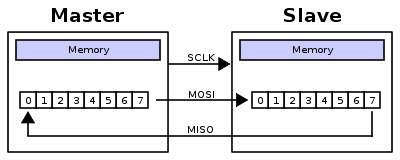
\includegraphics[width=0.5\textwidth]{SPI_8-bit_circular_transfer}
  	\caption{SPI Schieberegister Master-Slave}
  	\label{fig:SPI_Shift}
\end{figure}
Der Vorteil des \ac{spi} ist sein Vollduplex Modus, welcher durch Schieberegister in Slave und Master realisiert wird (siehe Abb. \ref{fig:SPI_Shift}). Für die Datenübertragung ergeben sich 4 verschiedene Modi, welche sich durch einstellen der \textit{Clock Polarity (CPOL)} und der \textit{Clock Phase (CPHA)} ergeben (siehe Tab. \ref{tab:spi_modes}). 
\begin{figure}[h!]
\centering
\begin{tikztimingtable}[timing/d/background/.style={fill=white},
   timing/lslope=0.2]
          CPOL=0 & LL 15{T} LL \\
          CPOL=1 & HH 15{T} HH \\
                 & H 17L H     \\
  \\
        Cycle \# & U     R 8{2Q} 2U    \\
            MISO & D{z}  R 8{2Q} 2D{z} \\
            MOSI & D{z}  R 8{2Q} 2D{z} \\
  \\
        Cycle \# & UU    R 8{2Q} U    \\
            MISO & D{z}U R 8{2Q} D{z} \\
            MOSI & D{z}U R 8{2Q} D{z} \\
\extracode
  % Add vertical lines in two colors
  \begin{pgfonlayer}{background}
    \begin{scope}[semitransparent,semithick]
      \vertlines[red]{2.1,4.1,...,17.1}
      \vertlines[blue]{3.1,5.1,...,17.1}
    \end{scope}
  \end{pgfonlayer}
  % Add big group labels
  \begin{scope}
    [font=\sffamily\Large,shift={(-6em,-0.5)},anchor=east]
    \node at (  0, 0) {SCK};    \node at (  0,-3 ) {CS};
    \node at (1ex,-9) {CPHA=0}; \node at (1ex,-17) {CPHA=1};
  \end{scope}
\end{tikztimingtable}
\caption{\acs{spi} Datenübertragung mit unterschiedlichen Einstellungen}
\end{figure}
\begin{table}[h!]
\centering
\caption{\ac{spi} Modi Einstellungen}
\label{tab:spi_modes}
\begin{tabular}{c|c|c}
\textbf{Mode} & \textbf{Clock Polarity} & \textbf{Clock Phase} \\
\cline{1-3}
0	& 0	& 0 \\ 
1	& 0	& 1 \\ 
2	& 1	& 0 \\ 
3	& 1	& 1 \\ 
\end{tabular}
\end{table}
%
%
%
\subsection{Paralleles Dateninterface}\label{subsec:interface_parallel}
Für die Realisierung eines parallelen Dateninterfaces wird mindestens eine Datenleitung, welche die eigentliche Information des Bits enthält, sowie eine Taktleitung, welche den Schreibbefehl initialisiert, benötigt. Dabei kann die Anzahl an Datenleitungen variieren. In diesem Layout wurde sich für ein 8-bit breites Interface entschieden, da dieses mit einen Takt von 16 \ac{mhz} betrieben werden soll. Somit könnte eine theoretische Datenrate von 16 MB/s\footnote{$16\cdot 10^6$ Byte} realisiert werden, was zwar nicht die theoretischen 60 MB/s\footnote{480 MBit/s} der High-Speed \ac{usb} 2.0 Schnittstelle ausreizt, jedoch 160 32-Bit Werte bei einer \ac{prf} mit 12 \ac{khz} übertragen kann. Somit kann die Datenrate um 400 \% in Bezug auf die vorangestellte Arbeit gesteigert werden und bietet durch eine Busverbreitung auf 16 bit eine theoretische Datenrate von 32 MB/s.\\
%Serienwiderstände für die Reduzierung des Ringings wurden bei dieser Übertragungsfrequenz vernachlässigt.
Für die Synchronisierung der Daten wurde sich der Technik der PAL video Synchronisierung bedient. Dabei handelt es sich um ein zusätzliches Signal, welches den Spannungspegel bei Übertragung eines Pakets ändert. Mit dieser Technik können die übertragenen Werte einer \ac{prf} zugeordnet werden, was dem Empfänger die weitere Verarbeitung der Werte erleichtert. Somit entfällt eine sonst notwendige Nachbearbeitung durch Zuordnung von Start- und Stopbits des Transfers. Diese Erweiterung reduziert die \ac{mcu} Last des Empfängers, wodurch diesem mehr Zeit für andere Aufgaben \ac{resp} Berechnungen zu Verfügung stehen.
%
%
%
\newcounter{wavenum}

\setlength{\unitlength}{1cm}
% advance clock one cycle, not to be called directly
\newcommand*{\clki}{
  \draw (t_cur) -- ++(0,.3) -- ++(.5,0) -- ++(0,-.6) -- ++(.5,0) -- ++(0,.3)
    node[time] (t_cur) {};
}

\newcommand*{\bitvector}[3]{
  \draw[fill=#3] (t_cur) -- ++( .1, .3) -- ++(#2-.2,0) -- ++(.1, -.3)
                         -- ++(-.1,-.3) -- ++(.2-#2,0) -- cycle;
  \path (t_cur) -- node[anchor=mid] {#1} ++(#2,0) node[time] (t_cur) {};
}

% \known{val}{length}
\newcommand*{\known}[2]{
    \bitvector{#1}{#2}{white}
}

% \unknown{length}
\newcommand*{\unknown}[2][XXX]{
    \bitvector{#1}{#2}{black!20}
}

% \bit{1 or 0}{length}
\newcommand*{\bit}[2]{
  \draw (t_cur) -- ++(0,.6*#1-.3) -- ++(#2,0) -- ++(0,.3-.6*#1)
    node[time] (t_cur) {};
}

% \unknownbit{length}
\newcommand*{\unknownbit}[1]{
  \draw[ultra thick,black!50] (t_cur) -- ++(#1,0) node[time] (t_cur) {};
}

% \nextwave{name}
\newcommand{\nextwave}[1]{
  \path (0,\value{wavenum}) node[left] {#1} node[time] (t_cur) {};
  \addtocounter{wavenum}{-1}
}

% \clk{name}{period}
\newcommand{\clk}[2]{
    \nextwave{#1}
    \FPeval{\res}{(\wavewidth+1)/#2}
    \FPeval{\reshalf}{#2/2}
    \foreach \t in {1,2,...,\res}{
        \bit{\reshalf}{1}
        \bit{\reshalf}{0}
    }
}

% \begin{wave}[clkname]{num_waves}{clock_cycles}
\newenvironment{wave}[3][Dataclock]{
  \begin{tikzpicture}[draw=black, yscale=.7,xscale=1]
    \tikzstyle{time}=[coordinate]
    \setlength{\unitlength}{0.5cm}
    \def\wavewidth{#3}
    \setcounter{wavenum}{0}
    \nextwave{#1}
    \foreach \t in {0,1,...,\wavewidth}{
    %  \draw[dotted] (t_cur) +(0,.5) node[above] {t=\t} -- ++(0,.4-#2);
      \clki
    }
}{\end{tikzpicture}}


\begin{figure}[h!]
\centering
\begin{wave}{3}{5}
 \nextwave{Dataline[0\ldots 7]}	\bit{0}{0.5} \known{}{1}\known{}{1}\known{}{1}\known{}{1}\known{}{1} \bit{0}{0.5}
 \nextwave{Dataframe} 		\bit{0}{0.5} \bit{1}{5} \bit{0}{0.5}
\end{wave}
\caption{Datenübertragung eines Frames mit der parallelen Schnittstelle}
\end{figure}

%
%
%
\subsection{Fast Fourier Transformation}
Die \ac{fft} ist eine Methode, welche Daten aus dem Zeitbereich in den Frequenzbereich überführt.\newline
Diese Methode beruht auf einen Algorithmus, welcher die Eingangswerte vertauscht. Dabei wird in jedem Schritt das Abtastintervall zwischen zwei Werten verdoppelt. Dies wird solange wiederholt, bis alle Eingangswerte in 2-er Gruppen gespaltet sind. Dies hat zur Folge, dass für die \ac{fft} immer ein ganzzahliges Vielfaches der Auflösungsfrequenz korrekt ermittelbar ist.\newline
Die \ac{dft} benötigt \textbf{$N^2$} und die \ac{fft} \textbf{$N*log_{2}(N)$} Berechnungen. Somit werden für einen Zeitbereich von \ac{zb} $10^9$ ns für die \ac{fft} $\approx 30$ s und die \ac{dft} $\approx 31.2$ Jahre benötigt. \newline
Aus der Anzahl $N$ der Punkte und der Abtastfrequenz $f_A$ ist der Linienabstand im Frequenzbereich mit $\dfrac{f_A}{N}$ berechenbar. Weiterhin ist zu beachten, dass die \ac{fft} spiegelsymmetrisch zur Mitte ist und somit nur die Frequenzen von $k=0$ bis $k=\frac{N}{2}$ betrachtet werden und die k-te Frequenz $f_k$ durch $f_k=f*\dfrac{f_A}{N}$ definiert ist.